\section{Man against machine}
\label{sect:mam_study}
Here we set an experienced human scheduler up against a series of automated schedulers to see who wins.
description - likely problems assumptions errors how handled, input forms, what they did - notes from subject, how measured, results-comparison with other schedulers.

\subsection{Rational and introduction}
Selecting appropriate groups to perform is a complex task. There are many trade-offs to be made between the various competing preferences and constraints. When the schedule is heavily loaded, i.e. there are potentially more observations to perform than could be accomodated even under ideal conditions, the job of the scheduler becomes extremely difficult. A major problem is to determine just what those tradeoffs are - i.e. just how much more important is a high priority, non-urgent group relative to a medium priority urgent group?. It is because it is difficult to quantify these relative weights that we turn to the human scheduler. A human makes these sort of trade-offs on a daily basis - often with little knowledge they are doing it - if we set a human up to perform the task we might be able to deduce from what they have done and the choices they have made some of the rules they are using (often without realizing) and the relative weighting they employ. Additionally it was thought that it would be useful just to know if a human was in fact capable of \emph{beating} an automated scheduler in terms of the standard SQMs.

\subsection{Methodology}
Describe here that we perform 2 sets of experiments. Firstly the human scheduler - no details yet these go in the intro to the experiment. Secondly a set of simulations where we fiddle with weights to try and reproduce the results of H1 or ideally beat them.


\subsection{Characterization of problem}
Plots of dmd and contention for the problem plus any relevant tabulated information.

\begin{figure}[htbp]
\begin{center}
    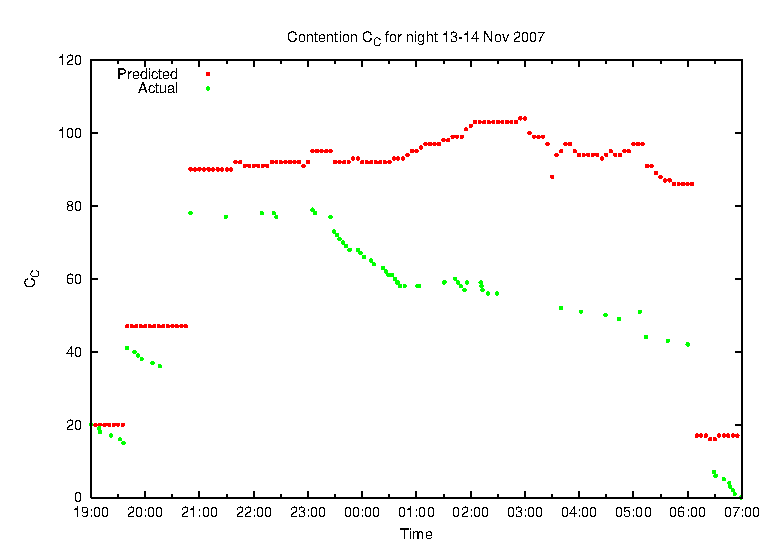
\includegraphics[scale=1.0, angle=0]{figures/mam/cont.eps}
\end{center}
\caption[Contention for night 13-14 November 2007.]
{Contention for night 13-14 November 2007 for H1 test. The two plots show the expected contention based on ODB content calculated in advance and the actual contention derived during a typial scheduling run on the night.}
\label{fig:mam_h1_contention}
\end{figure}

\begin{figure}[htbp]
\begin{center}
    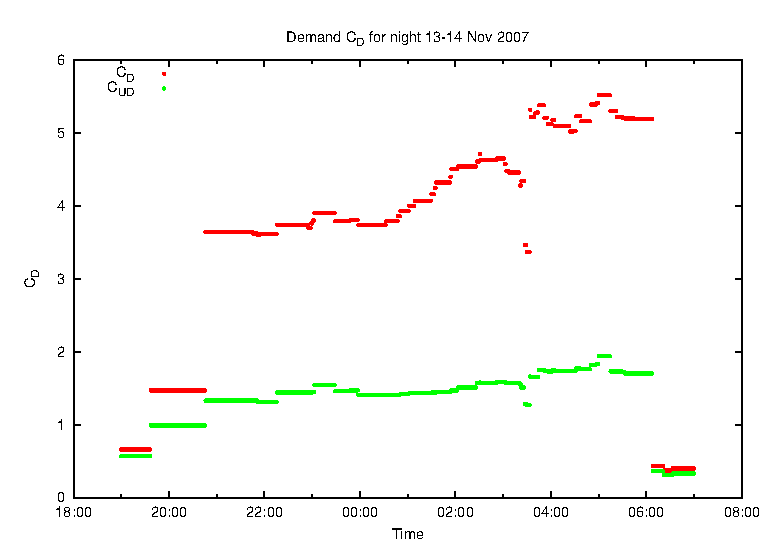
\includegraphics[scale=1.0, angle=0]{figures/mam/dmd.eps}
\end{center}
\caption[Demand for night 13-14 November 2007.]
{Demand for night 13-14 November 2007 for H1 test. The two plots show the overall and urgency-weighted demand.}
\label{fig:mam_h1_dmd}
\end{figure}

\subsection{Method of presentation}
What information is presented to the human scheduler.
A human subject (expert scheduler) is provided with information concerning which groups are potentially feasible on the test night. The information (described below) contains details of the target, timing and observing contsraints along with a pre-calculated feasibility plot for the night for each group. Some metrics are also available:- the urgency metric indicates on how many remaining nights the group might be observed, the exec-time metric indicates the expected execution time of the group. The HS then uses the information to devise a schedule for the night by recording the start time and ID of each group to execute in order.
The resulting schedule file is then read by an seperate analysis application to determine whether the schedule is actually feasible and, if so, generates the various quality metrics.

\begin{table}
\begin{center}
\begin{tabular}{|l|l|l|l|l|l|l|l|l|l|l|}
\hline
{\bf Column} & {\bf Title}  & {\bf Example} & {\bf Description}\\
\hline
1  & Numeric ID     & G\_476      & Group numeric ID. These are generated IDs which the HS uses to mark up the proposed schedule.\\
2  & Target RA      & 0:42:49.64  & The RA of the target in hh:mm:ss format\\
3  & Target Dec     & 41:15:26.50 & The declination of the target in dd:mm:ss format.\\
4  & Group Name     & ANGM31      & The actual name of the group.\\
5  & Timing         & MONITR 2.5H [2] & Class and detail e.g. Monitor 12h, Interval 48h.\\
6  & Moon OC        &             & Whether the group can be observed with the moon risen.\\
7  & Seeing OC      & POOR        & Which minimum seeing category the group can be observed in.\\
8  & Solar Elev OC  &             & Whether the group can be observed in twilight conditions.\\
9  & Priority       & 2           & The TAG assigned priority of this group (0-5, background, std).\\
10 & Execution Time & 33.4M       & How long the group is expected to take to run.\\
11 & Urgency        & CRIT        & Pre-calculated urgency - number of remaining nights the group can be observed.\\
12 & Availability   &             & A simple pre-calculated display of group observability during the night. \\
G\_476  &0:42:49.64&41:15:26.50  &ANGM31  &MONITR 2.5H [2]    &     &POOR  &       &2 &33.4M   &CRIT  \\
\hline

\end{tabular}
\label{tab:hsgexample}
\caption{Example output from HumanSchedulerTestGenerator}
\end{center}
\end{table}

In light of the difficulty for a human to generate the schedule by collating the considerable amount of information available a number of the normal constraints were relaxed. e.g. it is not easy for a human to keep precise track of the accumulating time to the second so execution times are given to the nearest minute. The accuracy of the availability plot is also shown to around 5-10 minutes so when testing the feasibility (in terms of target elevation) a few degrees of leeway are given. In order to uncomplicate the scenario the assumption is made that seeing is good for the whole night. The analysis proceeds as follows:
For each scheduled group, time pair, the feasibility is worked out for that time (this consists of testing the target elevation against dome limit (20 degs)) and the group constraints on moon and sun elevation against actual elevations. If feasible then the various quality metrics are computed. The results are summed and output. Due to the time taken to perform one of these HS trials - several hours, only a single trial was performed.

Tables of crit and non-crit groups. What fields in table - explain what they are.
Explain how the human is restricted and how we relax some constraints e.g. elevation limit as HS cannot work this out easily for any given time.

\clearpage

\begin{landscape}
\tiny
\begin{verbatim}
000 GROUP G_279     0:51:21.75   20:55:56.10  Star_H01            MONITR 168H [167]                   POOR ASTR  P= BGR XT= 2.53M    RN= 7    *********5____
000 GROUP G_361     0:51:21.75   20:55:56.10  Focus01_rr          INTVAL 168H                         AVER CIVT  P= BGR XT= 9.8M     RN= 18   *********5____
000 GROUP G_362     0:51:21.75   20:55:56.10  Focus01_Har         INTVAL 12H                          AVER CIVT  P= BGR XT= 12.1M    RN= ICRT *********5____
000 GROUP G_363     0:51:21.75   20:55:56.10  Focus01_gr          INTVAL 1H                           AVER CIVT  P= BGR XT= 9.9M     RN= ICRT *********5____
000 GROUP G_364     0:51:21.75   20:55:56.10  Focus01_ir          INTVAL 12H                          AVER CIVT  P= BGR XT= 9.9M     RN= ICRT *********5____
000 GROUP G_368     0:51:21.75   20:55:56.10  Focus01_Vr          INTVAL 12H                          AVER CIVT  P= BGR XT= 9.9M     RN= ICRT *********5____
000 GROUP G_375     0:42:49.64   41:15:26.50  Angstrom            MONITR 24H [18]                     POOR       P= 3   XT= 8.7M     RN= CRIT *********9____
000 GROUP G_399     0:49:48.00   32:16:43.00  887g000t000         FLEXBL                         DARK POOR       P= 2   XT= 3.27M    RN= 15   *********8____
000 GROUP G_423     0:43:29.48   41:17:13.50  M31b                MONITR 24H [18]                     POOR       P= 2   XT= 12.6M    RN= CRIT *********9____
000 GROUP G_446     0:58:59.80   1:0:10.00    gals_to_calib_3     FLEXBL                         DARK AVER       P= 1   XT= 36.07M   RN= 14   ********9_____
000 GROUP G_461     0:50:19.00   24:30:32.00  UCM_galaxies_5      FLEXBL                         DARK AVER       P= 1   XT= 39.63M   RN= 14   *********5____
000 GROUP G_476     0:42:49.64   41:15:26.50  ANGM31              MONITR 2.5H [2]                     POOR       P= 2   XT= 33.4M    RN= CRIT *********9____
000 GROUP G_059     1:42:20.00   51:34:32.00  925a000t000         FLEXBL                         DARK POOR       P= 1   XT= 3.27M    RN= 15   ***********3__
000 GROUP G_101     1:24:48.00   9:32:21.00   923g000t000         FLEXBL                         DARK POOR       P= 1   XT= 3.27M    RN= 11   *********6____
000 GROUP G_159     1:50:42.00   21:45:35.00  923j000t000         FLEXBL                         DARK POOR       P= 3   XT= 3.27M    RN= 13   9*********5___
000 GROUP G_319     1:34:25.49   30:21:47.30  M33_cal_chip31      FLEXBL                              POOR       P= 2   XT= 17.47M   RN= 18   **********5___
000 GROUP G_323     1:34:16.08   30:31:9.90   M33_cal_chip22      FLEXBL                              POOR       P= 2   XT= 17.47M   RN= 18   **********5___
000 GROUP G_324     1:33:22.75   30:18:26.80  M33_cal_chip33      FLEXBL                              POOR       P= 2   XT= 17.47M   RN= 18   **********4___
\end{verbatim}
\end{landscape}
\normalsize



%\begin{landscape}
%\tiny
%\begin{table}
%\begin{center}
%\begin{tabular}{|l|l|l|l|l|l|l|l|l|l|l|}
%\hline
%{\bf ID} & {\bf RA}    & {\bf Dec} & {\bf Name} & {\bf Timing} & {\bf Moon}  & {\bf Seeing} & {\bf Night}   & {\bf Priority}    & {\bf Exec}   & {\bf Urgency} \\
%\hline
%G\_448  &22:41:55.90  &20:15:42.00  &UCM\_galaxies\_6&FLEXBL  &DARK &AVER  &       &1 &39.63M  &11 \\
%\hline
%G\_449  &23:51:25.70  &24:24:12.00  &UCM\_galaxies\_18&FLEXBL &DARK &AVER  &       &1 &39.63M  &12 \\
%\hline
%G\_450  &23:22:20.90  &23:0:42.00&UCM\_galaxies\_14  &FLEXBL  &DARK &AVER  &       &1 &39.63M  &12 \\
%\hline
%G\_452  &22:58:50.00  &20:17:54.00  &UCM\_galaxies\_7&FLEXBL  &DARK &AVER  &       &1 &39.63M  &11 \\
%\hline
%G\_453  &23:31:48.50  &24:44:6.00&UCM\_galaxies\_17  &FLEXBL  &DARK &AVER  &       &1 &39.63M  &12 \\
%\hline
%G\_455  &23:5:25.50&21:9:42.00&UCM\_galaxies\_4&FLEXBL        &DARK &AVER  &       &1 &39.63M  &12  \\
%\hline
%G\_466  &22:53:57.74  &16:8:53.56&2251  &MONITR 168H [167]    &DARK &AVER  &       &1 &7.8M   &2  \\
%\hline
%G\_469  &22:2:43.291  &42:16:39.98  &2200 &MONITR 168H [167]  &     &AVER  &       &1 &7.8M   &2 \\
%\hline
%G\_470  &2:38:38.93&16:36:59.28  &0235 &MONITR 168H [167]     &DARK &AVER  &       &1 &7.8M   &2  \\
%\hline
%G\_471  &12:29:6.70&2:3:8.60  &1226 &MONITR 168H [167]        &     &AVER  &       &1 &7.8M   &2  \\
%\hline
%G\_472  &8:54:48.90&20:6:30.64&0851 &MONITR 168H [167]        &DARK &AVER  &       &1 &7.8M   &2  \\
%\hline
%G\_476  &0:42:49.64&41:15:26.50  &ANGM31  &MONITR 2.5H [2]    &     &POOR  &       &2 &33.4M   &CRIT  \\
%\hline
%G\_481  &14:17:59.60  &25:6:53.00&5548\_opt&MONITR 168H [120] &     &POOR  &ASTR   &2 &3.13M  &3  \\
%\hline
%\end{tabular}
%\label{tab:hsgexample}
%\caption{Example output from HumanSchedulerTestGenerator}
%\end{center}
%\end{table}
%\normalsize
%\end{landscape}

\subsection{HS results}
Table of HS results for various metrics.

\subsection{Method of simulation}
Explain how we perform the simulations - cut-down architecture to mimic the information available to the HS. ie the automatic scheduler knows what the human knows.

\subsection{BDS simulation results}

\begin{table}
\begin{center}
\begin{tabular}{|l|rrrrrrrrr|}
\hline
{\bf metric} & {\bf $h_1$} & {\bf $B_{el}$} &  {\bf $B_{pr}$} & {\bf $B_{rn}$} & {\bf $B_{td}$} & {\bf $B_{2,8}$} & {\bf $B_{5,5}$} & {\bf $B_{8,2}$} & {\bf $B_{rnd}$}\\
\hline
{\bf $Q_{el}$} & 0.77 & 0.88 & 0.52 & 0.36 & 0.4  & 0.59 & 0.59 & 0.72 & 0.56 \\
{\bf $Q_{pr}$} & 2.34 & 1.87 & 2.29 & 1.73 & 1.54 & 2.3  & 2.3  & 2.16 & 1.43 \\
{\bf $Q_{sm}$} & 0.28 & 0.3  & 0.26 & 0.28 & 0.32 & 0.25 & 0.25 & 0.25 & 0.33 \\
{\bf $Q_{lm}$} & 0.71 & 0.8  & 0.68 & 0.82 & 0.92 & 0.64 & 0.64 & 0.7  & 0.86 \\
{\bf $Q_{rn}$} & 0.67 & 0.48 & 0.4  & 0.58 & 0.4  & 0.47 & 0.47 & 0.45 & 0.35 \\
{\bf $Q_{td}$} & 0.07 & 0.06 & 0.05 & 0.1  & 0.12 & 0.06 & 0.06 & 0.05 & 0.08 \\
{\bf $Q_{xt}$} & 0.99 & 0.99 & 0.96 & 0.99 & 1.0  & 0.96 & 0.97 & 0.96 & 1.0  \\
\hline
\end{tabular}
\label{tab:hsbdscomp}
\caption{Results of BDS simulations and Human scheduler}
\end{center}
\end{table}


\subsection{LAS simulation results}
extra features - bg selection thresh - other wise stay idle, overun thresh frac of group in horizon
\begin{table}
\begin{center}
\begin{tabular}{|l|r|rrrr|rrrr|rrrr|}
\hline
{\bf metric} & {\bf $h_1$} & {\bf 1} & {\bf 2} &  {\bf 4} & {\bf 8} & {\bf 1} & {\bf 2} &  {\bf 4} & {\bf 8}   & {\bf 1} & {\bf 2} &  {\bf 4} & {\bf 8} \\
\hline
EL & 0.77 & 0.574 &0.569 &0.579 &0.571 &0.569 &0.576 &0.584 &0.584 &0.573 &0.577 & 0.58 & 0.582\\
\hline
PR & 2.34 & 1.848 &1.801 &1.811 &1.812 &1.863 &1.818 &1.790 &1.807 &1.855 &1.826 & x&y\\
\hline
LM & 0.71 & 0.815 &0.820 &0.847 &0.839 &0.816 &0.831 &0.838 &0.843 &0.837 &0.838 & x&y\\
\hline
SM & 0.28 & 0.317 &0.321 &0.325 &0.327 &0.311 &0.326 &0.329 &0.330 &0.324 &0.327 & x&y\\
\hline
RN & 0.67 & 0.362 &0.344 &0.347 &0.358 &0.345 &0.357 &0.356 &0.344 &0.340 &0.342 & x&y\\
\hline
XT & 0.99 & 1.000 &0.998 &1.012 &1.007 &0.994 &1.010 &1.016 &1.011 &1.013 &1.011 & x&y\\
\hline
\end{tabular}
\label{tab:lascomp}
\caption{Results of LAS simulations and Human scheduler}
\end{center}
\end{table}

\subsection{Conclusions}
